\subsection{3. 可逆效应与反应性余效应}\label{revertible-efects-and-reactive-coefects}

本节把第~2~节引入的效应与余效应概念提升为运行时机制，构建一套动态组合理论。核心思想是把承载效应与余效应的类型上下文转化为上下文类型，即一种可在运行时操作、将上下文具体化为头等实体的类型。对于效应类型，我们将其建模为配对了逆变换的上下文变换，从而实现局部的时序可组合性；对于余效应上下文，我们将其建模为携带依赖信息的类型，从而实现局部的空间可组合性。余效应上的观测等价性随后为效应赋予独立性。同时承载效应与余效应的统一上下文本身，即构成一种独立的编程范式。

\subsection{3.1. 可逆效应}\label{revertible-efects}

时序可组合性是指在运行时加载与卸载组件的能力，使得在卸载时共享环境恢复到组合前的状态。这要求组件对环境的每一次修改既可追踪又可恢复。因此，我们把效应建模为类型为
\(\Gamma \to \Gamma \times ( \Gamma \to \Gamma )\)
的函数：将其作用于当前上下文，会得到修改后的上下文以及一个显式的逆变换。提供该逆变换使效应可以被逆转，而把它交还运行时则使效应可被追踪。我们称此类效应为可逆效应：通过在执行过程中追踪并复合这些逆变换，完整的环境恢复便成为一种结构性保证。

\subsection{3.1.1. 效应上下文}\label{efect-context}

对任意非纯函数 \(f _ { \mathrm { i m p u r e } } : X \to Y\)，我们将其变换为纯形式
\(f : \Gamma \times X \to \Gamma \times Y\)，其中 $\Gamma$ 是上下文，所有可能的副作用都可以表示为 $\Gamma$ 上的变换。对任意固定的输入 \(x : X\)，诱导映射
\(\gamma \mapsto \operatorname { p r } _ { 1 } ( f ( \gamma , x ) )\)
独立于返回值地捕获了 \(f\) 的副作用。因此，$\Gamma$ 上的效应存在于变换 $\Gamma \to \Gamma$ 在复合 \(\circ\) 下构成的幺半群中，其中每条幺半群公理都可以直接读作效应的一条性质：

• 封闭性：两个效应的顺序复合仍然是效应；

• 结合性：复合效应与括号的括法无关；

• 单位元：\({ \mathrm { i d } } _ { \Gamma }\)，即 $\Gamma$ 上的恒等函数，充当复合的单位元。

为了建模可以撤销的效应，我们把每个变换 \(f\) 与另一个撤销 \(f\) 的变换 \(g\) 配对，并称 \(g\) 为 \(f\) 的左逆，在全文简称为逆。撤销是单向的：逆需要满足的是 \(g \circ f\)，而从不要求 \(f \circ g\)。变换对自身也带有一个乘法运算：

定义 1. 定义上下文变换对的扭曲复合为

\[
( f _ { 1 } , g _ { 1 } ) \circ ( f _ { 2 } , g _ { 2 } ) : = ( f _ { 1 } \circ f _ { 2 } , g _ { 2 } \circ g _ { 1 } )\tag{4}
\]

与 \(\circ\) 本身一样，左操作数在右操作数之后作用，逆变换按相反顺序累积。这使
\(( \Gamma \to \Gamma ) \times ( \Gamma \to \Gamma )\) 构成幺半群，其单位元为
\(( \mathrm { i d } _ { \Gamma } , \mathrm { i d } _ { \Gamma } )\)，即变换幺半群与其反向的直积，我们称之为 $\Gamma$ 上的扭曲复合幺半群 \(\mathfrak { T } _ { \Gamma }\)。

为了在上下文内部追踪效应，我们引入如下定义：

定义 2. 给定上下文 $\Gamma$，定义其效应上下文为：

\[
\partial \Gamma : = \Gamma \times ( \Gamma \to \Gamma )\tag{5}
\]

它可以理解为一个二元组 \(( \gamma , \varphi )\)，其中：

• \(\gamma : \Gamma\) 是当前上下文状态；

• \(\varphi : \Gamma \to \Gamma\) 是累加器，即迄今已执行的各效应之逆的复合，也是把上下文恢复到其初始状态的函数。

特别地，初始效应上下文可以表示为
\(( \gamma _ { 0 } , \mathrm { i d } _ { \Gamma } )\)。

我们还记
\(\partial ^ { 2 } \Gamma = \partial \Gamma \times ( \partial \Gamma \to \partial \Gamma )\)，以此逐层向上。

由于累加器 \(\varphi\) 的存在，在 \(\partial \Gamma\) 上执行的所有效应都可以被追踪并恢复。下面我们给出追踪与恢复的具体构造。

定义 3. 定义上下文函数对上的变换 \(\operatorname { t r a c k } _ { \Gamma }\)：

\[
\begin{array} { l r c l c l c }
  { \operatorname { t r a c k } _ { \Gamma } } & { \colon } & { ( \Gamma \to \Gamma ) \times ( \Gamma \to \Gamma ) } & { \to } & { \partial \Gamma } & { \to } & { \partial \Gamma } \\
  { \operatorname { t r a c k } _ { \Gamma } } & { = } & { ( f , g ) } & { \mapsto } & { ( \gamma , \varphi ) } & { \mapsto } & { ( f ( \gamma ) , \varphi \circ g ) }
\end{array}\tag{6}
\]

该变换把前向函数 \(f\) 连同候选逆变换 \(g\) 转化为效应上下文 \(\partial \Gamma\) 上的一个变换。将
\(\operatorname { t r a c k } _ { \Gamma } ( f , g )\) 作用于状态 \(( \gamma , \varphi )\) 会以 \(f\) 变换 \(\gamma\)，并把逆变换 \(g\) 复合到 \(\varphi\) 上，从而在上下文中追踪 \(f\) 的效应。

定理 4. 对任意
\(( f , g ) \in ( \Gamma \to \Gamma ) \times ( \Gamma \to \Gamma )\)，下图交换，即

\[
\mathrm { p r } _ { 1 } \circ \mathrm { t r a c k } _ { \Gamma } ( f , g ) = f \circ \mathrm { p r } _ { 1 }\tag{7}
\]

\pandocbounded{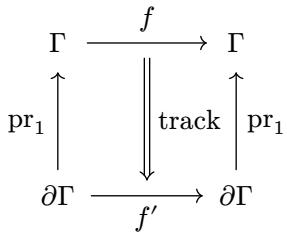
\includegraphics[keepaspectratio,alt={image}]{images/6ccf2193f4307249863af49c1bc005e170202baab7e50db5b126edc1426dfbe5.jpg}}

证明. 对所有 \(( \gamma , \varphi ) \in \partial \Gamma\)，

\[
\begin{array} { r }
  { ( \mathrm { p r } _ { 1 } \circ \mathrm { t r a c k } _ { \Gamma } ( f , g ) ) ( \gamma , \varphi ) = \mathrm { p r } _ { 1 } ( f ( \gamma ) , \varphi \circ g ) } \\
  { = f ( \gamma ) } \\
  { = ( f \circ \mathrm { p r } _ { 1 } ) ( \gamma , \varphi ) }
\end{array}
\]

定理 5. \(\operatorname { t r a c k } _ { \Gamma }\) 是从 \(\mathfrak { T } _ { \Gamma }\) 到
\(\partial \Gamma \to \partial \Gamma\) 的幺半群同态。即：

\begin{enumerate}
\def\labelenumi{\arabic{enumi}.}
\item
  \(\operatorname { t r a c k } _ { \Gamma } ( \mathrm { i d } _ { \Gamma } , \mathrm { i d } _ { \Gamma } ) = \mathrm { i d } _ { \partial \Gamma } ;\)
\item
  对所有
  \(( f _ { 1 } , g _ { 1 } ) , ( f _ { 2 } , g _ { 2 } ) \in \mathfrak { T } _ { \Gamma }\)，
\end{enumerate}

\[
\operatorname { t r a c k } _ { \Gamma } ( ( f _ { 1 } , g _ { 1 } ) \circ ( f _ { 2 } , g _ { 2 } ) ) = \operatorname { t r a c k } _ { \Gamma } ( f _ { 1 } , g _ { 1 } ) \circ \operatorname { t r a c k } _ { \Gamma } ( f _ { 2 } , g _ { 2 } )\tag{8}
\]

证明.

\begin{enumerate}
\def\labelenumi{\arabic{enumi}.}
\item
  单位元被映为单位元，因为
  \(\operatorname { t r a c k } _ { \Gamma } ( \mathrm { i d } _ { \Gamma } , \mathrm { i d } _ { \Gamma } ) ( \gamma , \varphi ) = ( \gamma , \varphi \circ \mathrm { i d } _ { \Gamma } ) = ( \gamma , \varphi )\)。
\item
  对乘法，取任意 \(( \gamma , \varphi ) \in \partial \Gamma\)。
\end{enumerate}

\[
\begin{array} { r l }
  & ( \operatorname { t r a c k } _ { \Gamma } ( f _ { 1 } , g _ { 1 } ) \circ \operatorname { t r a c k } _ { \Gamma } ( f _ { 2 } , g _ { 2 } ) ) ( \gamma , \varphi ) = \operatorname { t r a c k } _ { \Gamma } ( f _ { 1 } , g _ { 1 } ) ( f _ { 2 } ( \gamma ) , \varphi \circ g _ { 2 } ) \\
  & \qquad = ( f _ { 1 } ( f _ { 2 } ( \gamma ) ) , \varphi \circ g _ { 2 } \circ g _ { 1 } ) \\
  & \qquad = \operatorname { t r a c k } _ { \Gamma } ( f _ { 1 } \circ f _ { 2 } , g _ { 2 } \circ g _ { 1 } ) ( \gamma , \varphi )
\end{array}
\]

定义 6. 定义 \(\partial \Gamma\) 上的变换 \(\operatorname { r e c o v e r } _ { \Gamma }\)：

\[
\begin{array} { l r c l }
  { \operatorname { r e c o v e r } _ { \Gamma } } & { \colon } & { \partial \Gamma } & { \to \quad \partial \Gamma } \\
  { \operatorname { r e c o v e r } _ { \Gamma } } & { = } & { ( \gamma , \varphi ) } & { \mapsto ( \varphi ( \gamma ) , \mathrm { i d } _ { \Gamma } ) }
\end{array}\tag{9}
\]

该变换把恢复函数 \(\varphi\) 应用于当前状态 \(\gamma\)，并把 \(\varphi\) 重置为恒等函数。下图说明在效应序列
\(\operatorname { t r a c k } ( f _ { 1 } , g _ { 1 } ) , \cdots , \operatorname { t r a c k } ( f _ { n } , g _ { n } )\)
被应用于 \(\partial \Gamma\) 之后，recover 如何把上下文恢复到其初始状态：

\[
\begin{array} { r l }
  & \Gamma \xrightarrow { f _ { 1 } } \Gamma \longrightarrow \cdots \longrightarrow \Gamma \xrightarrow { f _ { n } } \Gamma \\
  & \Bigg \Updownarrow \mathrm { t r a c k } \qquad \qquad \qquad \qquad \Bigg \downarrow \mathrm { t r a c k } \\
  & \partial \Gamma \xrightarrow { f _ { 1 } ^ { \prime } } \partial \Gamma \longrightarrow \cdots \longrightarrow \partial \Gamma \xrightarrow { f _ { n } ^ { \prime } } \partial \Gamma \\
  & \Bigg \uparrow \qquad \qquad \qquad \qquad \qquad \mathrm { r e c o v e r }
\end{array}
\]

该图表明，被追踪的效应与随后的 recover 把初始效应上下文带回其自身。每一步追踪所保持的，正是从任意状态出发执行恢复所得的结果：

定理 7. 对任意 \(( \gamma , \varphi ) \in \partial \Gamma\) 以及满足
\(g ( f ( \gamma ) ) = \gamma\) 的任意对 \(( f , g )\)，

\[
\operatorname { r e c o v e r } _ { \Gamma } \bigl ( \operatorname { t r a c k } _ { \Gamma } ( f , g ) ( \gamma , \varphi ) \bigr ) = \operatorname { r e c o v e r } _ { \Gamma } ( \gamma , \varphi )\tag{10}
\]

证明.

\[
\begin{array} { r l }
  & \operatorname { r e c o v e r } _ { \Gamma } ( \operatorname { t r a c k } _ { \Gamma } ( f , g ) ( \gamma , \varphi ) ) = \operatorname { r e c o v e r } _ { \Gamma } ( f ( \gamma ) , \varphi \circ g ) \\
  & \qquad = ( \varphi ( g ( f ( \gamma ) ) ) , \mathrm { i d } _ { \Gamma } ) \\
  & \qquad = ( \varphi ( \gamma ) , \mathrm { i d } _ { \Gamma } ) = \operatorname { r e c o v e r } _ { \Gamma } ( \gamma , \varphi )
\end{array}
\]

对于成对的序列无需单独的论证。设 \(( f _ { 1 } , g _ { 1 } ) , \cdots , ( f _ { n } , g _ { n } )\) 从
\(( \gamma , \varphi )\) 出发按顺序施加，并记 \(\delta _ { 0 } = \gamma\) 与
\(\delta _ { i } : = f _ { i } ( \delta _ { i - 1 } )\)。由定理~5，复合追踪
\(\operatorname { t r a c k } _ { \Gamma } ( f _ { n } , g _ { n } ) \circ \cdots \circ \operatorname { t r a c k } _ { \Gamma } ( f _ { 1 } , g _ { 1 } )\)
正是扭曲复合
\(( f _ { n } \circ \cdots \circ f _ { 1 } , g _ { 1 } \circ \cdots \circ g _ { n } )\)
的追踪，并且若对每个 \(i\) 都有 \(g _ { i } ( \delta _ { i } ) = \delta _ { i - 1 }\)，则
\(( g _ { 1 } \circ \cdots \circ g _ { n } ) ( \delta _ { n } ) = \delta _ { 0 } = \gamma\)。
因此该对在 \(\gamma\) 处满足定理~7 的假设，应用一次该定理即得

\[
\operatorname { r e c o v e r } _ { \Gamma } ( ( \operatorname { t r a c k } _ { \Gamma } ( f _ { n } , g _ { n } ) \circ \dotsb \circ \operatorname { t r a c k } _ { \Gamma } ( f _ { 1 } , g _ { 1 } ) ) ( \gamma , \varphi ) ) = \operatorname { r e c o v e r } _ { \Gamma } ( \gamma , \varphi )\tag{11}
\]

取 \(( \gamma , \varphi ) = ( \gamma _ { 0 } , \mathrm { i d } _ { \Gamma } )\)，恢复会把按此方式到达的每个状态都带回
\(( \gamma _ { 0 } , \mathrm { i d } _ { \Gamma } )\)。满足 \(g \circ f = \operatorname { i d } _ { \Gamma }\) 的对在每个状态处都满足该假设。

恢复通过量 \(\varphi ( \gamma )\) 读取状态，我们把 \(\varphi ( \gamma ) = \gamma _ { 0 }\) 称为 \(\partial \Gamma\) 中状态的可靠性不变量。

\subsection{3.1.2. 可逆效应函数}\label{revertible-efect-functions}

上一节的 track/recover 模型把逆变换视为先验给定的：\(\operatorname { t r a c k } _ { \Gamma } ( f , g )\) 在看到任何上下文状态之前就固定了 \(g\)，因此同一个 \(g\) 必须服务于效应施加处的每个状态。然而在实践中，每个效应的逆变换并非先验可知：它必须由调用者在效应施加点提供。此外，recover 是全有或全无的：它无法在保留其他效应的同时选择性地撤销某一个。为解决这两个问题，我们在输入侧与输出侧同时增强该模型：

\begin{enumerate}
\def\labelenumi{\arabic{enumi}.}
\item
  在输入侧，我们不仅变换 $\Gamma$，还随之返回一个逆变换函数，使得逆变换在效应施加处被提供：\(\Gamma \to \Gamma \times ( \Gamma \to \Gamma )\)，即
  \(\Gamma \to \partial \Gamma\)；
\item
  在输出侧，我们不仅变换 \(\partial \Gamma\)，还随之返回一个逆变换函数，使得一个效应可以在保留其他效应的同时被撤销：\(\partial \Gamma \to \partial \Gamma \times ( \partial \Gamma \to \partial \Gamma )\)，即
  \(\partial \Gamma \to \partial ^ { 2 } \Gamma\)。
\end{enumerate}

这种增强保持了输入与输出之间结构上的一致性，因此我们仍能定义相应的理论，以维持 track 的数学性质。由此得到的类型是效应函数 \(\mathfrak { E } _ { \Gamma }\) 及其带见证的精化版本
\({ \mathfrak { E } } _ { \Gamma } ^ { * }\)：

定义 8. 定义效应函数 \(\mathfrak { E } _ { \Gamma }\) 与见证效应函数
\({ \mathfrak { E } } _ { \Gamma } ^ { * }\)：

\[
\begin{array} { r l }
  & \mathfrak { E } _ { \Gamma } : = \Gamma \to \Gamma \times ( \Gamma \to \Gamma ) \\
  & \mathfrak { E } _ { \Gamma } ^ { * } : = \big ( e : \Gamma \to \Gamma \times ( \Gamma \to \Gamma ) \big ) \\
  & \quad \quad \times \big ( ( \gamma : \Gamma ) \to ( ( \delta : \Gamma ) \times ( g : \Gamma \to \Gamma ) \times ( ( \delta , g ) = e ( \gamma ) \to g ( \delta ) = \gamma ) ) \big )
\end{array}\tag{12}
\]

其中 \(e ( \gamma )\) 产生一个二元组 \(( \delta , g )\)，表示：

• \(\delta : \Gamma\) 是新的上下文；

• \(g : \Gamma \to \Gamma\) 是当前效应的逆变换函数。

\(\mathfrak { E } _ { \Gamma } ^ { * }\) 中的元素按状态选择其逆变换，约束 \(g ( \delta ) = \gamma\) 把该选择限定为在效应被施加处逆转效应，而在其他任何地方都不对 \(g\) 施加约束。满足
\(g \circ f = \operatorname { i d } _ { \Gamma }\) 的单个 \(g\) 同时满足每个状态处的约束，并通过
\(( f , g ) \mapsto \gamma \mapsto ( f ( \gamma ) , g )\) 诱导出 \(\mathfrak { E } _ { \Gamma } ^ { * }\) 中的一个元素，定理~11 将证明这是一个同态。该约束可以可视化为如下交换图，确保逆变换 \(g\) 确实在 \(e\) 被施加的状态处反转该变换：

\pandocbounded{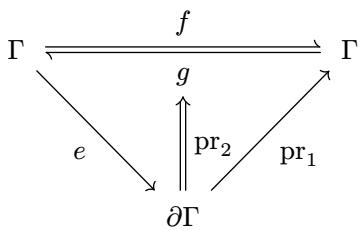
\includegraphics[keepaspectratio,alt={image}]{images/f2d6628215cd6fc08d01d2447a4d8728b73398e933b83424d748e2e755d79cc5.jpg}}

由于效应函数 \(\mathfrak { E } _ { \Gamma }\) 不再是上下文上的自同态，它们无法直接复合。因此我们为效应复合定义一个新的运算：

定义 9. 给定函数 \(f , g \in \mathfrak { E } _ { \Gamma }\)，定义它们的效应复合 \(f \diamond g\)：

\[
\begin{array} { l r c l }
  { f \diamond g } & { \colon } & { \Gamma } & { \to \partial \Gamma } \\
  { f \diamond g } & { = } & { \gamma } & { \mapsto \mathbf { l e t } \ ( \delta , s ) = g ( \gamma ) \ \mathbf { i n } \ \mathbf { l e t } \ ( \varepsilon , t ) = f ( \delta ) \ \mathbf { i n } \ ( \varepsilon , s \circ t ) }
\end{array}\tag{13}
\]

定理 10. 效应复合把 \(\mathfrak { T } _ { \Gamma }\) 的幺半群结构迁移到
\(\mathfrak { E } _ { \Gamma }\) 上。即：

\begin{enumerate}
\def\labelenumi{\arabic{enumi}.}
\item
  \(( \mathfrak { E } _ { \Gamma } , \diamond )\) 是幺半群，其单位元为
  \(\eta _ { \Gamma } : = \gamma \mapsto ( \gamma , \mathrm { i d } _ { \Gamma } ) ;\)
\item
  赋值 \(( f , g ) \mapsto \gamma \mapsto ( f ( \gamma ) , g )\) 是从 \(\mathfrak { T } _ { \Gamma }\) 到
  \(\mathfrak { E } _ { \Gamma }\) 的幺半群同态。
\end{enumerate}

证明.

\begin{enumerate}
\def\labelenumi{\arabic{enumi}.}
\item
  结合律与单位元定律按分量直接由 \(\circ\) 的相应性质得到。
\item
  记 \(e _ { i } = \gamma \mapsto ( f _ { i } ( \gamma ) , g _ { i } )\)；则
  \(( e _ { 1 } \diamond e _ { 2 } ) ( \gamma ) = ( f _ { 1 } ( f _ { 2 } ( \gamma ) ) , g _ { 2 } \circ g _ { 1 } )\)，
  即 \(\left( f _ { 1 } , g _ { 1 } \right) \circ \left( f _ { 2 } , g _ { 2 } \right)\) 的像，且
  \(( \mathrm { i d } _ { \Gamma } , \mathrm { i d } _ { \Gamma } )\) 映到 \(\eta _ { \Gamma }\)。□
\end{enumerate}

定理 11. 见证在效应复合下保持不变，且一致逆变换在每个状态处都构成见证。即：

\begin{enumerate}
\def\labelenumi{\arabic{enumi}.}
\item
  \(\mathfrak { E } _ { \Gamma } ^ { * }\) 是 \(\mathfrak { E } _ { \Gamma }\) 的子幺半群；
\item
  定理~10 中的同态把每个满足 \(g \circ f = \operatorname { i d } _ { \Gamma }\) 的对都映入
  \(\mathfrak { E } _ { \Gamma } ^ { * }\)。
\end{enumerate}

证明.

\begin{enumerate}
\def\labelenumi{\arabic{enumi}.}
\item
  单位元位于 \(\mathfrak { E } _ { \Gamma } ^ { * }\) 中，因为
  \(\operatorname { i d } _ { \Gamma } ( \gamma ) = \gamma\)。对封闭性，取
  \(f , g \in \mathfrak { E } _ { \Gamma } ^ { * }\) 及任意 \(\gamma \in \Gamma\)，设
  \(( \delta , s ) = g ( \gamma )\)、\(( \varepsilon , t ) = f ( \delta )\)，于是
  \(( f \diamond g ) ( \gamma ) = ( \varepsilon , s \circ t )\)。那么
  \(s ( \delta ) = \gamma\) 且 \(t ( \varepsilon ) = \delta\)，从而
  \(( s \circ t ) ( \varepsilon ) = s ( \delta ) = \gamma\)。
\item
  \(g \circ f = \operatorname { i d } _ { \Gamma }\) 给出对每个 \(\gamma\) 有
  \(g ( f ( \gamma ) ) = \gamma\)，因此这类对的像在每个状态处都被见证。□
\end{enumerate}

正如 track 把 $\Gamma$ 上的一对变换提升到 \(\partial \Gamma\)，我们定义 effect 把
\(\mathfrak { E } _ { \Gamma }\) 提升到 \(\mathfrak { E } _ { \partial \Gamma }\)：

定义 12. 定义效应函数变换 \(\operatorname { e f f e c t } _ { \Gamma }\)：

\[
\begin{array} { l r c l c l }
  { \operatorname { e f f e c t } _ { \Gamma } } & { \colon } & { \mathfrak { E } _ { \Gamma } } & { \to } & { \partial \Gamma } & { \to \partial ^ { 2 } \Gamma } \\
  { \operatorname { e f f e c t } _ { \Gamma } } & { = } & { e } & { \mapsto } & { ( \gamma , \varphi ) } & { \mapsto \mathbf { l e t } \ ( \delta , g ) = e ( \gamma ) \ \mathbf { i n } \ ( ( \delta , \varphi \circ g ) , \operatorname { t r a c k } _ { \Gamma } ( g , \operatorname { p r } _ { 1 } \circ e ) ) }
\end{array}\tag{14}
\]

由于 \(\operatorname { e f f e c t } _ { \Gamma } ( e )\) 本身是 \(\mathfrak { E } _ { \partial \Gamma }\) 中的元素，它所返回的逆变换应按定义~8 高一层的意义来理解。该逆变换本身正是交换效应的两个方向所得之对的一个追踪。普通的追踪规则再次适用：撤销效应本身也是一个效应，它以 \(g\) 变换状态，而撤销它的方式就是再次执行该效应，这正是 \(\operatorname { p r } _ { 1 } \circ e\) 所做的。因此该逆变换复合到交给它的累加器上，恰如 track 所规定的那样。

我们现在可以证明 effect 与 track 相类似的性质。

定理 13. effect 保持 ⋄ 运算。即，对所有 \(f , g \in \mathfrak { E } _ { \Gamma }\)，

\[
\operatorname { e f f e c t } _ { \Gamma } ( f ) \diamond \operatorname { e f f e c t } _ { \Gamma } ( g ) = \operatorname { e f f e c t } _ { \Gamma } ( f \diamond g )\tag{15}
\]

证明. 取任意 \(( \gamma , \varphi ) \in \partial \Gamma\)，设
\(( \delta , s ) = g ( \gamma )\) 与 \(( \varepsilon , t ) = f ( \delta )\)，于是
\(( f \diamond g ) ( \gamma ) = ( \varepsilon , s \circ t )\)，且
\(\operatorname { p r } _ { 1 } \circ ( f \diamond g ) = ( \operatorname { p r } _ { 1 } \circ f ) \circ ( \operatorname { p r } _ { 1 } \circ g )\)。则

\[
\begin{array} { r l }
  & ( \operatorname { e f f e c t } _ { \Gamma } ( f ) \diamond \operatorname { e f f e c t } _ { \Gamma } ( g ) ) ( \gamma , \varphi ) = ( ( \varepsilon , \varphi \circ s \circ t ) , \operatorname { t r a c k } _ { \Gamma } ( s , \operatorname { p r } _ { 1 } \circ g ) \circ \operatorname { t r a c k } _ { \Gamma } ( t , \operatorname { p r } _ { 1 } \circ f ) ) \\
  & \qquad = ( ( \varepsilon , \varphi \circ s \circ t ) , \operatorname { t r a c k } _ { \Gamma } ( s \circ t , ( \operatorname { p r } _ { 1 } \circ f ) \circ ( \operatorname { p r } _ { 1 } \circ g ) ) ) \\
  & \qquad = \operatorname { e f f e c t } _ { \Gamma } ( f \diamond g ) ( \gamma , \varphi )
\end{array}
\]

其中第一步在 \(( \gamma , \varphi )\) 与 \(( \delta , \varphi \circ s )\) 处展开定义~12，第二步用到定理~5，第三步折叠定义~12。□

两个层次之间的关系由下图展示。其上三角是 \(e\) 的见证条件（按定义~8），其下三角则是
\(e ^ { \prime }\) 是否像 \(e\) 一样被见证的问题。

\pandocbounded{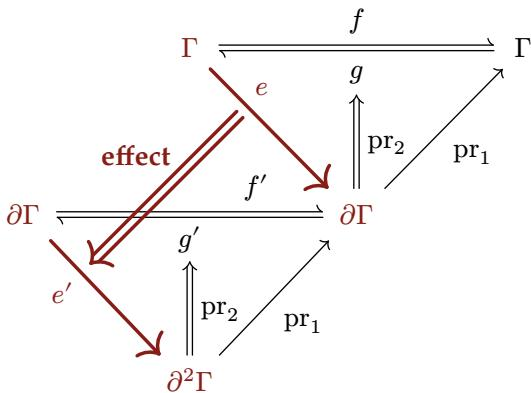
\includegraphics[keepaspectratio,alt={image}]{images/21186ec878faabc31d96dd91c90577b582af7acf8a5b61cde0f72d038f47fa16.jpg}}

在层次之间，投影 \(\operatorname { p r } _ { 1 }\) 把每个被提升的映射与其所提升的映射联系起来，正如它在定理~4 中为 track 所做的那样。

定理 14. 设 \(e \in \mathfrak { E } _ { \Gamma }\)，记 \(f : = \operatorname { p r } _ { 1 } \circ e\)，并令
\(e ^ { \prime } : = \operatorname { e f f e c t } _ { \Gamma } ( e )\)，其前向映射为
\(f ^ { \prime } : = \operatorname { p r } _ { 1 } \circ e ^ { \prime }\)。则

\begin{enumerate}
\def\labelenumi{\arabic{enumi}.}
\item
  \(\operatorname { p r } _ { 1 } \circ f ^ { \prime } = f \circ \operatorname { p r } _ { 1 } ;\)
\item
  对每个 \(( \gamma , \varphi ) \in \partial \Gamma\)，在该处被见证的提升逆变换
  \(g ^ { \prime } : = \operatorname { p r } _ { 2 } ( e ^ { \prime } ( \gamma , \varphi ) )\) 与逆变换
  \(g : = \operatorname { p r } _ { 2 } ( e ( \gamma ) )\) 满足
  \(\operatorname { p r } _ { 1 } \circ g ^ { \prime } = g \circ \operatorname { p r } _ { 1 }\)。
\end{enumerate}

证明.

\begin{enumerate}
\def\labelenumi{\arabic{enumi}.}
\item
  由定义~12，
  \(f ^ { \prime } ( \gamma , \varphi ) = ( f ( \gamma ) , \varphi \circ g )\)，
  其状态为
  \(f ( \gamma ) = ( f \circ \operatorname { p r } _ { 1 } ) ( \gamma , \varphi )\)。
\item
  这是对 \(g ^ { \prime } = \operatorname { t r a c k } _ { \Gamma } ( g , f )\) 应用定理~4。
\end{enumerate}

下三角是否闭合，可通过计算被提升的逆变换所返回的内容来确定：

定理 15. 设 \(e \in \mathfrak { E } _ { \Gamma } ^ { * }\)，记 \(f : = \operatorname { p r } _ { 1 } \circ e\)。固定
\(( \gamma , \varphi ) \in \partial \Gamma\)，设 \(( \delta , g ) = e ( \gamma )\)，并以
\(( \Delta , g ^ { \prime } )\) 表示 \(\operatorname { e f f e c t } _ { \Gamma } ( e )\) 在
\(( \gamma , \varphi )\) 处的值。则

\[
g ^ { \prime } ( \Delta ) = ( \gamma , \varphi \circ g \circ f )\tag{16}
\]

状态被精确恢复。累加器也被恢复——等价地，
\(\operatorname { e f f e c t } _ { \Gamma } ( e ) \in \mathfrak { E } _ { \partial \Gamma } ^ { * }\)——当且仅当
\(g \circ f = \operatorname { i d } _ { \Gamma }\)；并且在任何情况下都有
\(( \varphi \circ g \circ f ) ( \gamma ) = \varphi ( \gamma )\)，因此可靠性不变量得以保持。

证明. 由定义~12，\(\Delta = ( \delta , \varphi \circ g )\) 且
\(g ^ { \prime } = \operatorname { t r a c k } _ { \Gamma } ( g , f )\)，所以

\[
g ^ { \prime } ( \Delta ) = ( g ( \delta ) , \varphi \circ g \circ f ) = ( \gamma , \varphi \circ g \circ f )
\]

其中用到了 \(g ( \delta ) = \gamma\)。要属于 \(\mathfrak { E } _ { \partial \Gamma } ^ { * }\)，需对每个输入都等于
\(( \gamma , \varphi )\)；取 \(\varphi = \mathrm { i d } _ { \Gamma }\) 可把累加器的相等化为
\(g \circ f = \operatorname { i d } _ { \Gamma }\)，而该条件反过来又对每个 \(\varphi\) 给出累加器的相等。最后，
\(( \varphi \circ g \circ f ) ( \gamma ) = \varphi ( g ( \delta ) ) = \varphi ( \gamma )\)。□

因此，只有当在 \(\gamma\) 处被见证的逆变换在每个状态处都逆转 \(f\) 时，下三角才会闭合，所以
\(\operatorname { e f f e c t } _ { \Gamma }\) 不把 \(\mathfrak { E } _ { \Gamma } ^ { * }\) 映入
\(\mathfrak { E } _ { \partial \Gamma } ^ { * }\)。在任何情况下都成立的是在 \(\gamma\) 处的一致：
\(\operatorname { r e c o v e r } _ { \Gamma } ( g ^ { \prime } ( \Delta ) ) = \operatorname { r e c o v e r } _ { \Gamma } ( \gamma , \varphi )\)，这正是定理~7 对累加器所假设的全部内容，因此逆转不会触及恢复目标。

按施加顺序之逆序逆转效应无需任何额外条件，因为此时每个逆变换面对的正是其自身施加所产生的那个状态：

定理 16. 设 \(e _ { 1 } , \cdots , e _ { n } \in \mathfrak { E } _ { \Gamma } ^ { * }\) 从
\(( \gamma _ { 0 } , \mathrm { i d } _ { \Gamma } )\) 出发按顺序施加并按逆序逆转。则

\begin{enumerate}
\def\labelenumi{\arabic{enumi}.}
\item
  每次逆转都恢复其施加时所针对的上下文状态；
\item
  每个中间状态都满足可靠性不变量。
\end{enumerate}

证明. 每一步要么是一次施加，要么是一次逆转。一次施加把 \(( \gamma , \varphi )\) 带到
\(( \delta , \varphi \circ g )\)，其中 \(g ( \delta ) = \gamma\)，因此由定理~7 它保持
\(\varphi ( \gamma )\)，而定理~7 的假设正是 \(\mathfrak { E } _ { \Gamma } ^ { * }\) 的见证。按逆序逆转使每个逆变换面对其自身施加所产生的状态，因此由定理~15，该次逆转精确恢复前一个状态，并同样保持
\(\varphi ( \gamma )\)；这两个结论都不依赖于逆变换所接收到的累加器。□

\subsection{3.1.3. 效应的独立性}\label{independence-of-efects}

在效应自身施加所产生的状态下逆转它，是定理~16 所覆盖的情形；在其他任何状态下逆转它，则是本小节覆盖的情形。有两种情况需要后者。一种情况是逆变换在更晚的效应仍然在位时运行，这正相当于从运行中的系统中撤回一个组件；另一种情况是一个序列可以交错多个组件的效应，每个组件各自保留自己的逆变换，因此一个组件的逆变换被另一个组件的施加所分隔。在这两种情况下，逆变换所面对的状态都被外来效应移动过，而它是否仍能逆转它原本要逆转的内容，是一个交换性问题：需要交换的是，一个效应所能执行的每个变换与另一个效应所能执行的每个变换，前向映射与所产出的逆变换都一样。单独的累加器无法解决这两种情形，因为 \(\varphi\) 是一个复合，它以单一顺序一次性运行它所持有的每个逆变换。

定义 17. 对效应函数 \(e \in \mathfrak { E } _ { \Gamma }\)，变换幺半群
\(\mathfrak { M } ( e )\) 是由 \(e\) 的前向映射连同 \(e\) 产出的每个逆变换生成的
\(\Gamma \to \Gamma\) 的子幺半群，而 \(\mathfrak { M } ( e )\) 的生成元就是该生成集的元素：

\[
\mathfrak { M } ( e ) : = \langle \{ \mathrm { p r } _ { 1 } \circ e \} \cup \{ \mathrm { p r } _ { 2 } ( e ( \gamma ) ) \mid \gamma \in \Gamma \} \rangle\tag{17}
\]

由对 \(( f , g ) \in \mathfrak { T } _ { \Gamma }\) 诱导的效应以 \(f\) 与 \(g\) 为生成元，它在每个状态处产出的逆变换都是 \(g\)。

引理 18. 交换性在生成元上即可判定，且 ⋄ 不扩大任何变换幺半群。即：

\begin{enumerate}
\def\labelenumi{\arabic{enumi}.}
\item
  若 \(\mathfrak { M } ( e _ { 1 } )\) 的每个生成元都与 \(\mathfrak { M } ( e _ { 2 } )\) 的每个生成元交换，则
  \(\mathfrak { M } ( e _ { 1 } )\) 的每个元素都与 \(\mathfrak { M } ( e _ { 2 } )\) 的每个元素交换；
\item
  \(\mathfrak { M } ( e _ { 1 } \diamond e _ { 2 } ) \subseteq \langle \mathfrak { M } ( e _ { 1 } ) \cup \mathfrak { M } ( e _ { 2 } ) \rangle\)。
\end{enumerate}

证明.

\begin{enumerate}
\def\labelenumi{\arabic{enumi}.}
\item
  与 \(\mathfrak { M } ( e _ { 2 } )\) 的每个生成元交换的映射构成 \(\Gamma \to \Gamma\) 的一个子幺半群，因为
  \(\mathrm { i d } _ { \Gamma }\) 位于其中，且当 \(f\) 与 \(f ^ { \prime }\) 都在其中时
  \(f \circ f ^ { \prime }\) 也在其中。该子幺半群按假设包含 \(\mathfrak { M } ( e _ { 1 } )\) 的生成元，因而包含
  \(\mathfrak { M } ( e _ { 1 } )\)。固定 \(f \in \mathfrak { M } ( e _ { 1 } )\)，与 \(f\) 交换的映射同样构成一个子幺半群，它包含 \(\mathfrak { M } ( e _ { 2 } )\) 的生成元，因而包含
  \(\mathfrak { M } ( e _ { 2 } )\)。
\item
  由定义~9，\(e _ { 1 } \diamond e _ { 2 }\) 的前向映射是
  \(\left( \mathrm { p r } _ { 1 } \circ e _ { 1 } \right) \circ \left( \mathrm { p r } _ { 1 } \circ e _ { 2 } \right)\)，且它在任何状态处产出的逆变换都是 \(s \circ t\)，其中 \(s\) 由 \(e _ { 2 }\) 产出、\(t\) 由 \(e _ { 1 }\) 产出。因此
  \(\mathfrak { M } ( e _ { 1 } \diamond e _ { 2 } )\) 的每个生成元都是二者生成元的复合。□
\end{enumerate}

定义 19. 效应函数 \(e _ { 1 } , e _ { 2 } \in \mathfrak { E } _ { \Gamma }\) 当且仅当以下条件成立时称为独立的：

\begin{enumerate}
\def\labelenumi{\arabic{enumi}.}
\tightlist
\item
  其中一方的每个变换都与另一方的每个变换交换，
\end{enumerate}

\[
\forall f \in \mathfrak { M } ( e _ { 1 } ) , g \in \mathfrak { M } ( e _ { 2 } ) . \quad f \circ g = g \circ f\tag{18}
\]

\begin{enumerate}
\def\labelenumi{\arabic{enumi}.}
\setcounter{enumi}{1}
\tightlist
\item
  其中一方的变换都不扰动另一方所产出的逆变换，
\end{enumerate}

\[
\forall g \in \mathfrak { M } ( e _ { 2 } ) , \gamma \in \Gamma . \quad \mathrm { p r } _ { 2 } ( e _ { 1 } ( g ( \gamma ) ) ) = \mathrm { p r } _ { 2 } ( e _ { 1 } ( \gamma ) )\tag{19}
\]

并且交换 \(e _ { 1 }\) 与 \(e _ { 2 }\) 后同样成立。

族 \(\left( e _ { l } \right) _ { l \in L }\) 两两独立，是指对每个 \(l \neq l ^ { \prime }\)，\(e _ { l }\) 与
\(e _ { l ^ { \prime } }\) 都独立。一个族可以重复同一个效应函数，而使一个效应与自身独立，就是要使
\(\mathfrak { M } ( e )\) 交换。

对于由对 \(( f _ { 1 } , g _ { 1 } )\) 与 \(( f _ { 2 } , g _ { 2 } )\) 诱导的效应，条件 (1) 由引理~18(1) 等价于四对
\(f _ { 1 } , f _ { 2 }\)；\(g _ { 1 } , g _ { 2 }\)；\(f _ { 1 } , g _ { 2 }\)；与 \(g _ { 1 } , f _ { 2 }\) 的交换，而条件 (2) 直接成立，因为诱导效应在每个状态处只产出一个逆变换。在 ⋄ 下的交换是一个不同的性质。\(e _ { 1 } \diamond e _ { 2 } = e _ { 2 } \diamond e _ { 1 }\) 所等同的是：两种顺序下复合前向映射彼此相等，两种顺序下复合逆变换彼此相等，其中每个逆变换都在其自身施加所产生的状态处进入复合；独立性则把一方的每个变换与另一方的每个变换对应起来，包括前向映射与外来逆变换的配对。

在独立性下，逆变换可以在被更晚的效应移动过的状态处运行，而它在彼处撤回的只是自身的贡献，别无其他：

定理 20. 设 \(e _ { 1 } , \cdots , e _ { n } \in \mathfrak { E } _ { \Gamma } ^ { * }\) 两两独立，并从
\(\gamma _ { 0 }\) 出发按顺序施加。记 \(f _ { i } : = \mathbf { p r } _ { 1 } \circ e _ { i }\)，令
\(\delta _ { i } : = f _ { i } ( \delta _ { i - 1 } )\) 且 \(\delta _ { 0 } : = \gamma _ { 0 }\)，并令
\(g _ { i } : = \mathrm { p r } _ { 2 } ( e _ { i } ( \delta _ { i - 1 } ) )\) 为 \(e _ { i }\) 在施加处产出的逆变换。固定
\(j\)，记 \(\delta _ { i } ^ { \prime } : = \big ( f _ { i } \circ \cdots \circ f _ { j + 1 } \big ) \big ( \delta _ { j - 1 } \big )\) 为剔除 \(e _ { j }\) 后该序列的各状态，于是
\(\delta _ { j } ^ { \prime } = \delta _ { j - 1 }\)。则对每个满足 \(j \leq u \leq n\) 的 \(u\)：

\begin{enumerate}
\def\labelenumi{\arabic{enumi}.}
\item
  \(\delta _ { u } = f _ { j } ( \delta _ { u } ^ { \prime } )\) 且
  \(g _ { j } ( \delta _ { u } ) = \delta _ { u } ^ { \prime }\)；
\item
  每个满足 \(i > j\) 的 \(e _ { i }\) 在 \(\delta _ { i - 1 } ^ { \prime }\) 处产出的逆变换，与它在
  \(\delta _ { i - 1 }\) 处产出的逆变换相同，即 \(g _ { i }\)。
\end{enumerate}

证明.

\begin{enumerate}
\def\labelenumi{\arabic{enumi}.}
\tightlist
\item
  第一个等式是对 \(u\) 的归纳。在 \(u = j\) 处它读作
  \(\delta _ { j } = f _ { j } \big ( \delta _ { j - 1 } \big )\)，即 \(\delta _ { j }\) 的定义。对归纳步，
  \(\delta _ { u + 1 } = f _ { u + 1 } ( \delta _ { u } ) = f _ { u + 1 } ( f _ { j } ( \delta _ { u } ^ { \prime } ) ) = f _ { j } ( f _ { u + 1 } ( \delta _ { u } ^ { \prime } ) ) = f _ { j } \left( \delta _ { u + 1 } ^ { \prime } \right)\)，
  中间的等式用到定义~19 的条件 (1)，对 \(e _ { u + 1 }\) 与 \(e _ { j }\)，它们是该族中互异的效应，因为 \(u + 1 > j\)。对第二个等式，条件 (1) 把 \(g _ { j }\) 穿过在 \(e _ { j }\) 之后施加的前向映射带出来，把 \(e _ { j }\) 的见证留在它成立的那一个状态处使用：
\end{enumerate}

\[
g _ { j } ( \delta _ { u } ) = \bigl ( g _ { j } \circ f _ { u } \circ \cdots \circ f _ { j + 1 } \bigr ) \bigl ( \delta _ { j } \bigr ) = \bigl ( f _ { u } \circ \cdots \circ f _ { j + 1 } \bigr ) \bigl ( g _ { j } \bigl ( f _ { j } \bigl ( \delta _ { j - 1 } \bigr ) \bigr ) \bigr ) = \delta _ { u } ^ { \prime }
\]

最后一个等式依赖于
\(g _ { j } \big ( f _ { j } \big ( \delta _ { j - 1 } \big ) \big ) = \delta _ { j - 1 }\)，这是定义~8 要求 \(e _ { j }\) 在
\(\delta _ { j - 1 }\) 处满足的见证。

\begin{enumerate}
\def\labelenumi{\arabic{enumi}.}
\setcounter{enumi}{1}
\tightlist
\item
  由 (1)，状态 \(\delta _ { i - 1 }\) 是 \(f _ { j } ( \delta _ { i - 1 } ^ { \prime } )\)，且
  \(f _ { j } \in \mathfrak { M } ( e _ { j } )\)，因此对 \(e _ { i }\) 与 \(e _ { j }\) 应用定义~19 的条件 (2) 给出
  \(\mathrm { p r } _ { 2 } \big ( e _ { i } \big ( f _ { j } ( \delta _ { i - 1 } ^ { \prime } ) \big ) \big ) = \mathrm { p r } _ { 2 } \big ( e _ { i } ( \delta _ { i - 1 } ^ { \prime } ) \big )\)。□
\end{enumerate}

条件 (1) 定位了逆变换所到达的状态：即同一序列在该效应从未被施加的情况下本会到达的状态，无论其后施加了什么效应。条件 (2) 定位了其他效应在那里所持有的逆变换，二者合起来使该定理可以再次应用于更短的序列：

推论 21. 设 \(e _ { 1 } , \cdots , e _ { n } \in \mathfrak { E } _ { \Gamma } ^ { * }\) 两两独立，从
\(\gamma _ { 0 }\) 出发按顺序施加，并令 \(g _ { 1 } , \cdots , g _ { n }\) 如上。在 \(\delta _ { n }\) 处按
\(\{ 1 , \cdots , n \}\) 的任意排列的顺序施加这 \(n\) 个逆变换，都会到达 \(\gamma _ { 0 }\)。

证明. 对 \(n\) 向下归纳。设该排列以 \(j\) 开头。由定理~20(1)，在 \(\delta _ { n }\) 处施加 \(g _ { j }\) 到达
\(\delta _ { n } ^ { \prime }\)，即剔除 \(e _ { j }\) 后该序列所到达的状态，而由定理~20(2)，其余效应在那里产出的逆变换正是手中的 \(g _ { i }\)。该序列两两独立，因为它是子族，所以归纳假设适用于它以及排列的其余部分；空序列到达
\(\gamma _ { 0 }\)。□

LIFO 顺序正是这样一个排列，定理~16 在其中无需任何假设即可逆转。独立性带来的则是所有其他顺序，以及随之而来的交错多个组件的序列，第 4.4.2 节将其推广到整个系统的迹。

综上，这些构造共同构成可逆效应：\(\mathfrak { E } _ { \Gamma } ^ { * }\) 中的每个效应函数都显式地提供自身的逆变换，effect 在效应上下文 \(\partial \Gamma\) 上追踪这些逆变换，而 ⋄ 运算在保持可逆性的同时将它们复合。它们所带来的是局部的时序可组合性；所谓局部，是指该保证只针对单一组件的效应本身来解读。我们把它理解为如下准则：对于组件施加的每一个效应函数序列，累加器都恢复它所出发的上下文（定理~7），而逆转该序列时每个逆变换面对的正是其自身施加时所针对的状态（定理~16）。加载一个组件就是施加这样一个序列并把它的逆变换累积到 \(\varphi\) 中；卸载它就是施加 \(\varphi\)。

准则遗漏了两件事，而这两件事都在多个组件参与时才出现：脱离累加器所强加顺序的逆转，以及交错他人效应的序列。独立性提供了它们（推论~21），它是关于效应本身的一个条件，而非构造的性质；第 3.3.2 节识别了满足该条件的纪律，第 4.4.2 节则从整个系统的迹的角度解读该保证。当独立性不成立时，顺序必须由其他机制承担：在单一组件内部由累加器承担，无论效应为何，它都按 LIFO 顺序逆转（第 4.3.2 节）；跨组件则由声明式的余效应承担，它让一次激活对另一次激活排序（第 4.3.1 节）。
